\documentclass[10pt]{standalone}
\usepackage[utf8]{inputenc}
\usepackage{pgf,tikz,pgfplots}
\pgfplotsset{compat=1.15}
\usepackage{mathrsfs}
\usetikzlibrary{arrows}
\pagestyle{empty}
\begin{document}
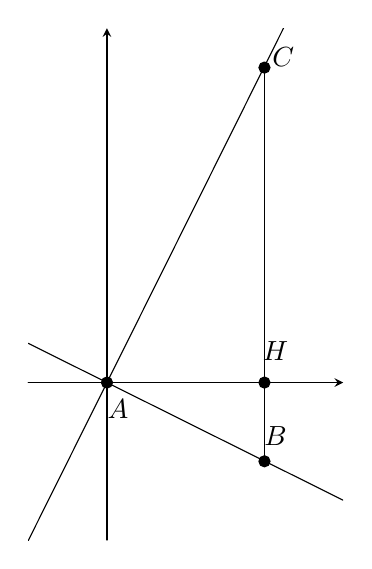
\begin{tikzpicture}[line cap=round,line join=round,>=triangle 45,x=1.0cm,y=1.0cm]
\begin{axis}[
x=1.0cm,y=1.0cm,
axis lines=middle,
xmin=-1.0,
xmax=3.0,
ymin=-2.0,
ymax=4.5,
xtick={-1.0,0.0,...,3.0},
ytick={-2.0,-1.0,...,5.0},
ticks=none]
\clip(-1.,-2.) rectangle (3.,5.);
\draw [domain=-1.:3.] plot(\x,{(-0.-2.78*\x)/5.58});
\draw [domain=-1.:3.] plot(\x,{(-0.--5.58*\x)/2.78});
\draw  (2.,4.)-- (2.0,-1.0);
\begin{scriptsize}

\draw [fill=black] (0.,0.) circle [radius=2.0pt];
\draw[color=black] (0.14,-0.33) node {$A$};

\draw [fill=black] (2.0,-1.0) circle [radius=2.0pt];
\draw[color=black] (2.14,-0.68) node {$B$};
\draw [fill=black] (2.0,0.0) circle [radius=2.0pt];
\draw[color=black] (2.14,0.4) node {$H$};
\draw [fill=black] (2.,4.) circle [radius=2.0pt];
\draw[color=black] (2.24,4.13) node {$C$};

\end{scriptsize}
\end{axis}
\end{tikzpicture}
\end{document}